% =====================================================================
%  MagneticTurk -- Data Sheet
%  Compile: pdflatex magneticturk_datasheet.tex   (run twice for contents)
%  Cover image: save a photo as cover.png / cover.jpg next to this file
%  and it replaces the placeholder automatically.
% =====================================================================
\documentclass[10pt,a4paper]{article}

\usepackage[a4paper,left=17mm,right=17mm,top=22mm,bottom=20mm,
            headheight=14pt,headsep=6mm,footskip=10mm]{geometry}
\usepackage[T1]{fontenc}
\usepackage[utf8]{inputenc}
\usepackage[scaled=0.92]{helvet}
\renewcommand{\familydefault}{\sfdefault}
\usepackage{microtype}

\usepackage{graphicx}
\usepackage{xcolor}
\usepackage{array,booktabs}
\usepackage{multicol}
\usepackage{enumitem}
\usepackage{fancyhdr}
\usepackage{titlesec}
\usepackage{titletoc}
\usepackage{caption}
\usepackage{siunitx}
\sisetup{mode=text,range-phrase=--}
\usepackage{ragged2e}
\usepackage{needspace}
\usepackage{etoolbox}
\usepackage{tikz}
\usetikzlibrary{positioning,arrows.meta,calc,fit,backgrounds,shapes.geometric,fadings}
\usepackage[hidelinks]{hyperref}

\newcommand{\product}{MagneticTurk}
\definecolor{brand}{HTML}{8C1D18}
\definecolor{grey}{HTML}{5A5A5A}
\definecolor{lightgrey}{HTML}{DDDDDD}
\definecolor{tint}{HTML}{F6F1F0}
\definecolor{coverdark}{HTML}{15171C}
\definecolor{brandlight}{HTML}{E0675E}

% ---------------------------------------------------------------- text
\setlength{\parindent}{0pt}
\setlength{\parskip}{4pt}
\setlength{\columnsep}{7mm}
\setlist{leftmargin=1.1em,itemsep=1.5pt,topsep=2pt,parsep=0pt}
\setlist[itemize]{label=\textbullet}
\setlist[enumerate]{leftmargin=1.5em,label=\textbf{\arabic*.}}

% ------------------------------------------------------------- headings
\pretocmd{\section}{\needspace{8\baselineskip}}{}{}
\pretocmd{\subsection}{\needspace{5\baselineskip}}{}{}
\titleformat{\section}{\large\bfseries}{\thesection}{0.7em}{}
  [\vspace{1pt}{\color{brand}\titlerule[0.6pt]}]
\titlespacing*{\section}{0pt}{12pt}{5pt}
\titleformat{\subsection}{\normalsize\bfseries}{\thesubsection}{0.7em}{}
\titlespacing*{\subsection}{0pt}{8pt}{2pt}

% ------------------------------------------------------ tables & figures
\captionsetup{labelfont=bf,font=small,labelsep=period,skip=4pt}
\renewcommand{\arraystretch}{1.3}
\newenvironment{simpletable}[1]
  {\par\addvspace{4pt}\noindent\begin{minipage}{\linewidth}\centering\captionof{table}{#1}\small
   \begin{tabular}{@{}>{\bfseries\RaggedRight\arraybackslash}p{0.32\linewidth}>{\RaggedRight\arraybackslash}p{0.62\linewidth}@{}}\toprule}
  {\bottomrule\end{tabular}\end{minipage}\par\addvspace{6pt}}

% Diagram styles
\tikzset{
  blk/.style={draw=black!70,fill=white,line width=0.6pt,rounded corners=1.2mm,
              align=center,inner sep=2.5mm,font=\footnotesize},
  key/.style={blk,draw=brand,line width=0.9pt,fill=tint},
  sub/.style={font=\scriptsize\color{grey}},
  lbl/.style={font=\scriptsize\color{grey},align=center,fill=white,inner sep=1pt},
  arr/.style={-{Stealth[length=2mm]},line width=0.6pt},
  barr/.style={{Stealth[length=2mm]}-{Stealth[length=2mm]},line width=0.6pt},
  pwr/.style={-{Stealth[length=2mm]},line width=0.9pt,color=brand},
  dec/.style={diamond,aspect=2.2,draw=black!70,fill=white,line width=0.6pt,
              align=center,inner sep=0.6mm,font=\footnotesize},
}
\newcommand{\bt}[2]{\textbf{#1}\\[-1pt]{\scriptsize\color{grey}#2}}

% -------------------------------------------------------- header/footer
\pagestyle{fancy}
\fancyhf{}
\fancyhead[L]{\small\bfseries\product{} \mdseries\color{grey}Data Sheet}
\fancyhead[R]{\small\color{grey}Frank Clarke \textbar{} October 2026}
\fancyfoot[R]{\small\bfseries\thepage}
\renewcommand{\headrule}{{\color{brand}\hrule height 0.8pt width\headwidth}}

% -------------------------------------------------------------- contents
\titlecontents{section}[1.8em]{\addvspace{4pt}\bfseries}
  {\contentslabel{1.8em}}{}{\titlerule*[0.6pc]{.}\contentspage}
\titlecontents{subsection}[4.2em]{\addvspace{1pt}}
  {\contentslabel{2.4em}}{}{\titlerule*[0.6pc]{.}\contentspage}

% =====================================================================
\begin{document}

% ============================== COVER ================================
\begin{titlepage}
\thispagestyle{empty}
\begin{tikzpicture}[remember picture,overlay]
  \def\panel{182mm}
  \coordinate (NW) at (current page.north west);
  \coordinate (PB) at ([yshift=-\panel]current page.north west);   % panel bottom-left
  \coordinate (PE) at ([yshift=-\panel]current page.north east);   % panel bottom-right

  % ---- dark panel
  \fill[coverdark] (NW) rectangle (PE);

  % ---- photo (fills the panel) or placeholder
  \IfFileExists{cover.png}{\def\coverfile{cover.png}}{%
  \IfFileExists{cover.jpg}{\def\coverfile{cover.jpg}}{\def\coverfile{}}}
  \ifx\coverfile\empty
    % placeholder: faint chessboard
    \begin{scope}[shift={([xshift=-124mm,yshift=-18mm]current page.north east)}]
      \foreach \i in {0,...,7}{\foreach \j in {0,...,7}{
        \ifodd\numexpr\i+\j\relax\else
          \fill[white,opacity=0.045] (\i*13mm,-\j*13mm) rectangle ++(13mm,-13mm);
        \fi}}
      \draw[white,opacity=0.12,line width=0.4pt] (0,0) rectangle (104mm,-104mm);
    \end{scope}
    \node[anchor=north east,font=\scriptsize,text=white,opacity=0.35]
      at ([xshift=-20mm,yshift=-125mm]current page.north east) {Product photo: save as cover.png};
  \else
    \begin{scope}
      \clip (NW) rectangle (PE);
      % scale to cover the whole panel, cropping the excess (no stretching)
      \sbox0{\includegraphics[width=\paperwidth]{\coverfile}}%
      \ifdim\ht0<\panel \sbox0{\includegraphics[height=\panel]{\coverfile}}\fi
      \node[inner sep=0,anchor=center] at ($(current page.north)+(0,-0.5*\panel)$) {\usebox0};
    \end{scope}
  \fi

  % ---- gradient so the title always reads, with or without a photo
  \fill[coverdark,path fading=north] (PB) rectangle ([yshift=110mm]PE);

  % ---- title block
  \node[anchor=south west,font=\footnotesize\bfseries,text=brandlight]
    at ([xshift=20mm,yshift=50mm]PB) {D\,A\,T\,A\enspace S\,H\,E\,E\,T};
  \node[anchor=south west,font=\fontsize{46}{48}\selectfont\bfseries,text=white]
    at ([xshift=19mm,yshift=27mm]PB) {\product};
  \node[anchor=south west,font=\Large,text=white!72]
    at ([xshift=20mm,yshift=15mm]PB) {Vision-guided chess-playing robotic arm};

  % ---- accent rule
  \fill[brand] (PB) rectangle ([yshift=-2.2mm]PE);

  % ---- summary + technologies
  \node[anchor=north west,text width=104mm,font=\large,align=left,inner sep=0]
    at ([xshift=20mm,yshift=-14mm]PB)
    {A robotic arm that plays chess on a real board. A camera on its wrist reads the position,
     Stockfish chooses the reply, and the arm picks up and places its own pieces, then checks with
     the camera that the move landed correctly.};
  \node[anchor=north west,text width=50mm,align=left,inner sep=0,font=\small]
    at ([xshift=-70mm,yshift=-14mm]PE)
    {{\footnotesize\bfseries\color{brand}TECHNOLOGIES}\\[2mm]
     Computer vision (OpenCV)\\[0.6mm]
     Inverse kinematics\\[0.6mm]
     Embedded Linux (Raspberry Pi)\\[0.6mm]
     I\textsuperscript{2}C servo control\\[0.6mm]
     Python, Stockfish, web interface};

  % ---- three facts
  \foreach \k/\num/\txt in {0/6/{servos driving five joints\\and a gripper},
                            1/64/{squares read by the camera\\every turn},
                            2/1/{Raspberry Pi running vision,\\chess and motion}}{
    \fill[brand] ([xshift=20mm+\k*58mm,yshift=-58mm]PB) rectangle ++(0.8mm,-15mm);
    \node[anchor=north west,inner sep=0,font=\fontsize{24}{26}\selectfont\bfseries]
      at ([xshift=24mm+\k*58mm,yshift=-57.5mm]PB) {\num};
    \node[anchor=north west,inner sep=0,font=\footnotesize,text=grey,align=left]
      at ([xshift=24mm+\k*58mm,yshift=-67mm]PB) {\txt};
  }

  % ---- footer
  \draw[lightgrey,line width=0.4pt] ([xshift=20mm,yshift=16mm]current page.south west)
    -- ([xshift=-20mm,yshift=16mm]current page.south east);
  \node[anchor=north west,font=\small\bfseries] at ([xshift=20mm,yshift=13mm]current page.south west) {Frank Clarke};
  \node[anchor=north east,font=\small,text=grey] at ([xshift=-20mm,yshift=13mm]current page.south east) {October 2026};
\end{tikzpicture}
\end{titlepage}

% ============================== CONTENTS =============================
\setcounter{page}{2}
{\Large\bfseries Contents}\par\vspace{2mm}
\noindent{\color{brand}\rule{\linewidth}{0.6pt}}\par\vspace{4mm}
\makeatletter\@starttoc{toc}\makeatother
\clearpage

% ============================== OVERVIEW =============================
\begin{multicols}{2}
\section{Overview}
\product{} is a robotic chess opponent that plays on a real board with ordinary pieces.
A six-servo robotic arm with a camera on its wrist reads the position, chooses a reply
with the Stockfish chess engine, and physically picks up and places its pieces, just
as a human player would.

After every move, the robot checks with the camera that the board matches the game
before handing the turn back. All of the vision, game logic and motion control runs on a
single Raspberry Pi. The chess clock, prompts and messages appear on any phone or
computer browser.

The key idea is that the camera is on the arm, so the robot can move to see better.
When it is unsure what it is looking at, it views the board again from a different angle,
and it uses the same approach to line up each grasp.

\subsection{Features}
\begin{itemize}
  \item Plays with real Staunton pieces, with no magnets or electronics in the board
  \item 6DOF metal arm: five joints plus a two-finger gripper
  \item Wrist-mounted \SI{12}{MP} autofocus camera
  \item Active vision: moves the camera to a better viewpoint whenever it is unsure
  \item Lines up each grasp visually before picking a piece
  \item Verifies every move, and retries or stops safely if something is wrong
  \item Stockfish engine with adjustable difficulty
  \item Supports captures, castling, en passant and promotion
  \item Chess clock and messages on a phone or computer
  \item Runs entirely on a Raspberry Pi Zero 2 W
\end{itemize}

\subsection{Applications}
\begin{itemize}
  \item Over-the-board play against an engine
  \item Practice at an adjustable playing strength
  \item Demonstrating robotics and computer vision
\end{itemize}

\subsection{Key Figures}
\begin{simpletable}{Typical performance}
Placement accuracy & About \SI{\pm 3}{mm}\\
Ordinary move      & About \SI{25}{s}\\
Capture            & About \SI{40}{s}\\
Reach              & All 64 squares and the capture tray\\
\end{simpletable}


\columnbreak
\section{How a Move Is Played}
Each turn follows the cycle in Figure~\ref{fig:cycle}. The robot never assumes a step
succeeded. It checks the board before acting and again afterwards.

\begin{center}
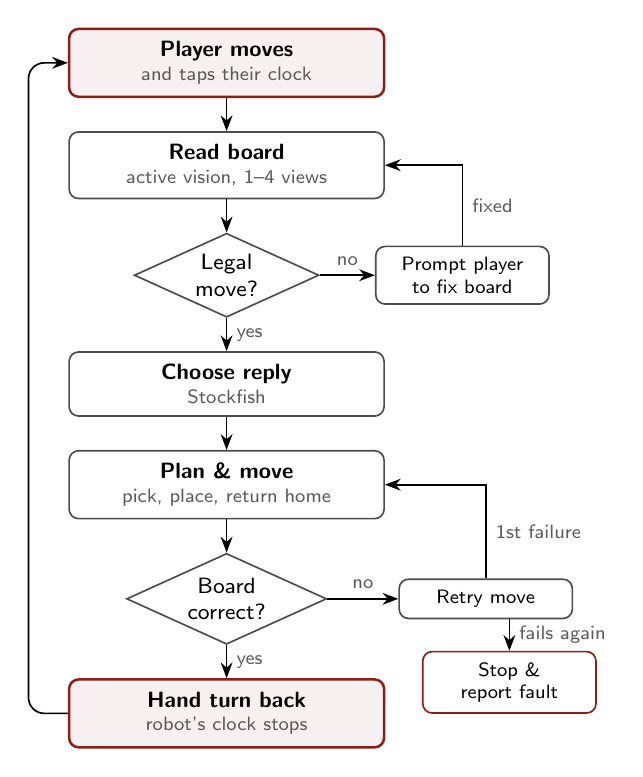
\begin{tikzpicture}[node distance=4.2mm,
  st/.style={blk,minimum width=40mm,inner sep=1.6mm},
  side/.style={blk,minimum width=22mm,inner sep=1.4mm,font=\scriptsize}]
  \node[key,minimum width=40mm,inner sep=1.6mm] (p) {\bt{Player moves}{and taps their clock}};
  \node[st,below=of p] (r) {\bt{Read board}{active vision, 1--4 views}};
  \node[dec,below=of r] (l) {Legal\\move?};
  \node[st,below=of l] (s) {\bt{Choose reply}{Stockfish}};
  \node[st,below=of s] (m) {\bt{Plan \& move}{pick, place, return home}};
  \node[dec,below=of m] (v) {Board\\correct?};
  \node[key,minimum width=40mm,inner sep=1.6mm,below=of v] (h) {\bt{Hand turn back}{robot's clock stops}};

  \node[side,right=7mm of l] (fix) {Prompt player\\to fix board};
  \node[side,right=9mm of v] (rt) {Retry move};
  \node[side,below=4mm of rt,draw=brand,xshift=3mm] (ft) {Stop \&\\report fault};

  \draw[arr] (p)--(r); \draw[arr] (r)--(l);
  \draw[arr] (l)--node[right,sub]{yes}(s); \draw[arr] (s)--(m); \draw[arr] (m)--(v);
  \draw[arr] (v)--node[right,sub]{yes}(h);
  \draw[arr] (l)--node[above,sub]{no}(fix);
  \draw[arr] (fix) |- node[sub,pos=0.25,right]{fixed} (r);
  \draw[arr] (v)--node[above,sub]{no}(rt);
  \draw[arr] (rt) |- node[sub,pos=0.25,right]{1st failure} (m);
  \draw[arr] (rt.south -| ft.north) -- node[sub,right]{fails again} (ft.north);
  \draw[arr,rounded corners=2mm] (h.west) -- ++(-5mm,0) |- (p.west);
\end{tikzpicture}
\captionof{figure}{Turn cycle}\label{fig:cycle}
\end{center}
\end{multicols}

% ======================== SYSTEM ARCHITECTURE (full width) ===========
\clearpage
\section{System Architecture}
The robot is built from off-the-shelf parts around a single Raspberry Pi Zero 2 W.
Figure~\ref{fig:hw} shows how the hardware is connected. Figure~\ref{fig:sw} shows how
the software turns a camera image into an arm movement and checks the result.

\begin{center}
\resizebox{\linewidth}{!}{%
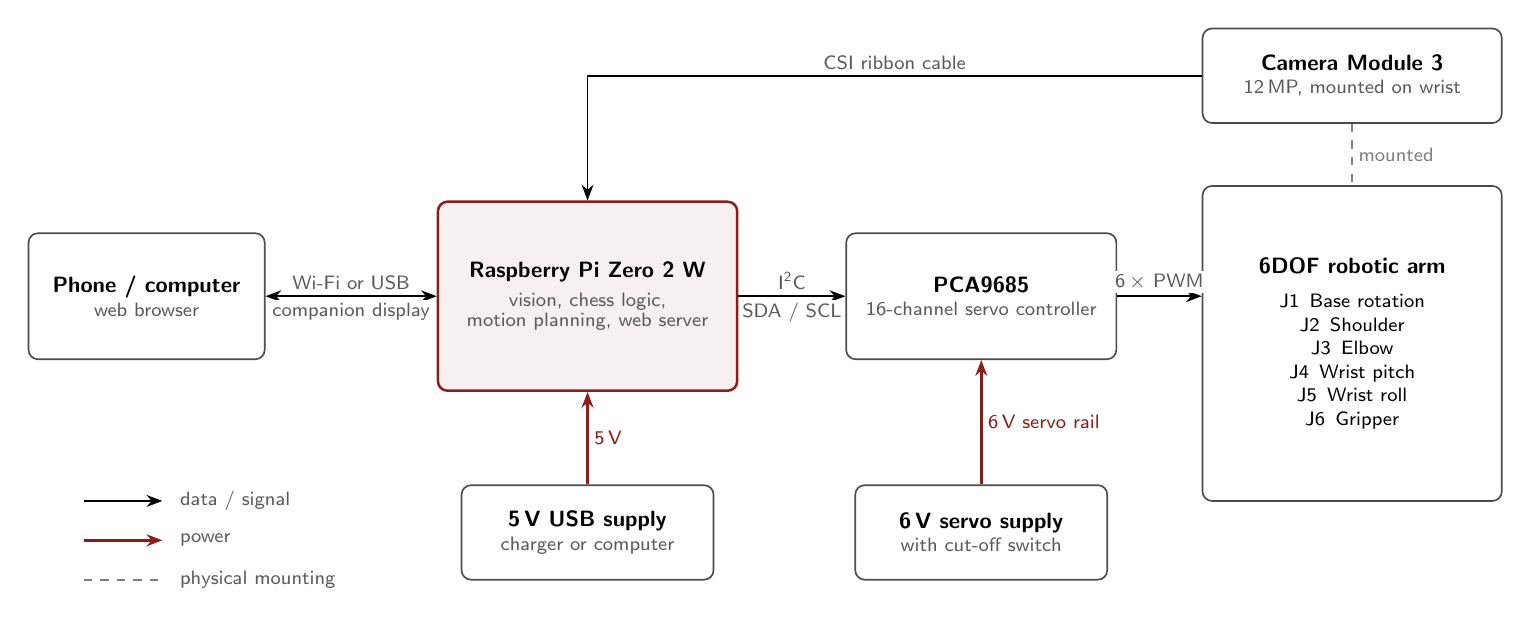
\begin{tikzpicture}[x=1mm,y=1mm]
  % main row
  \node[blk,minimum width=30mm,minimum height=16mm] (phone) at (-6,0)
       {\bt{Phone / computer}{web browser}};
  \node[key,minimum width=38mm,minimum height=24mm] (pi) at (50,0)
       {\textbf{Raspberry Pi Zero 2 W}\\[1pt]{\scriptsize\color{grey}vision, chess logic,}\\[-2pt]
        {\scriptsize\color{grey}motion planning, web server}};
  \node[blk,minimum width=32mm,minimum height=16mm] (pca) at (100,0)
       {\bt{PCA9685}{16-channel servo controller}};
  \node[blk,minimum width=38mm,minimum height=40mm,anchor=west] (arm) at (128,-6)
       {\textbf{6DOF robotic arm}\\[3pt]
        {\scriptsize J1\enspace Base rotation}\\[-1pt]
        {\scriptsize J2\enspace Shoulder}\\[-1pt]
        {\scriptsize J3\enspace Elbow}\\[-1pt]
        {\scriptsize J4\enspace Wrist pitch}\\[-1pt]
        {\scriptsize J5\enspace Wrist roll}\\[-1pt]
        {\scriptsize J6\enspace Gripper}};
  % camera on wrist
  \node[blk,minimum width=38mm,minimum height=12mm,anchor=west] (cam) at (128,28)
       {\bt{Camera Module 3}{12\,MP, mounted on wrist}};
  % supplies
  \node[blk,minimum width=32mm,minimum height=12mm] (usb) at (50,-30)
       {\bt{5\,V USB supply}{charger or computer}};
  \node[blk,minimum width=32mm,minimum height=12mm] (sps) at (100,-30)
       {\bt{6\,V servo supply}{with cut-off switch}};

  % data links
  \draw[barr] (phone) -- node[lbl,above=1pt]{Wi-Fi or USB} node[lbl,below=1pt]{companion display} (pi);
  \draw[arr] (pi) -- node[lbl,above=1pt]{I\textsuperscript{2}C} node[lbl,below=1pt]{SDA / SCL} (pca);
  \draw[arr] (pca.east) -- node[lbl,above=1pt]{6\,$\times$ PWM} (pca.east -| arm.west);
  \draw[arr] (cam.west) -- node[lbl,above=1pt]{CSI ribbon cable} (cam.west -| pi.north) -- (pi.north);
  \draw[dashed,line width=0.6pt,black!50] (cam.south) -- node[lbl,right=1pt]{mounted} (arm.north);
  % power
  \draw[pwr] (usb) -- node[lbl,right=1pt]{5\,V} (pi);
  \draw[pwr] (sps) -- node[lbl,right=1pt]{6\,V servo rail} (pca);

  % legend
  \begin{scope}[shift={(0,-30)}]
    \draw[arr] (-14,4) -- ++(10,0); \node[sub,anchor=west] at (-3,4) {data / signal};
    \draw[pwr] (-14,-1) -- ++(10,0); \node[sub,anchor=west] at (-3,-1) {power};
    \draw[dashed,black!50,line width=0.6pt] (-14,-6) -- ++(10,0); \node[sub,anchor=west] at (-3,-6) {physical mounting};
  \end{scope}
\end{tikzpicture}}
\captionof{figure}{Hardware block diagram. The servos are powered separately from the
Raspberry Pi, and all supplies share a common ground.}\label{fig:hw}
\end{center}

\vspace{4mm}
\begin{center}
\resizebox{\linewidth}{!}{%
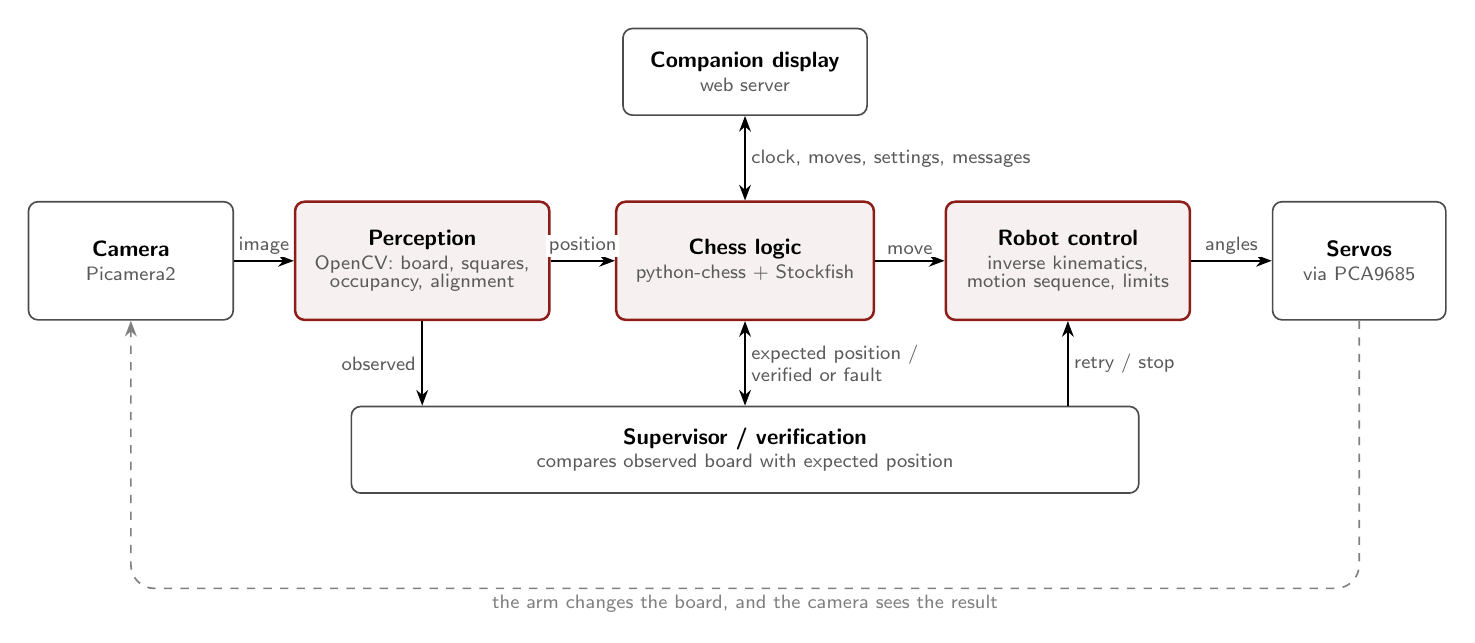
\begin{tikzpicture}[x=1mm,y=1mm]
  \node[blk,minimum width=26mm,minimum height=15mm] (cam) at (0,0) {\bt{Camera}{Picamera2}};
  \node[key,minimum width=31mm,minimum height=15mm] (per) at (37,0) {\bt{Perception}{OpenCV: board, squares,}\\[-3pt]{\scriptsize\color{grey}occupancy, alignment}};
  \node[key,minimum width=31mm,minimum height=15mm] (chs) at (78,0) {\bt{Chess logic}{python-chess + Stockfish}};
  \node[key,minimum width=31mm,minimum height=15mm] (rob) at (119,0) {\bt{Robot control}{inverse kinematics,}\\[-3pt]{\scriptsize\color{grey}motion sequence, limits}};
  \node[blk,minimum width=22mm,minimum height=15mm] (arm) at (156,0) {\bt{Servos}{via PCA9685}};

  \node[blk,minimum width=100mm,minimum height=11mm] (sup) at (78,-24) {\bt{Supervisor / verification}{compares observed board with expected position}};
  \node[blk,minimum width=31mm,minimum height=11mm] (web) at (78,24) {\bt{Companion display}{web server}};

  \draw[arr] (cam)--node[lbl,above=1pt]{image}(per);
  \draw[arr] (per)--node[lbl,above=1pt]{position}(chs);
  \draw[arr] (chs)--node[lbl,above=1pt]{move}(rob);
  \draw[arr] (rob)--node[lbl,above=1pt]{angles}(arm);
  \draw[arr] (per.south) -- node[lbl,left=1pt]{observed} (per.south |- sup.north);
  \draw[barr] (chs.south) -- node[lbl,right=1pt,align=left]{expected position /\\verified or fault} (chs.south |- sup.north);
  \draw[arr] (sup.north -| rob.south) -- node[lbl,right=1pt]{retry / stop} (rob.south);
  \draw[barr] (chs) -- node[lbl,right=1pt]{clock, moves, settings, messages} (web);
  \draw[arr,dashed,rounded corners=3mm,black!50] (arm.south) -- ++(0,-34) -| node[lbl,pos=0.25,below=1pt]{the arm changes the board, and the camera sees the result} (cam.south);
\end{tikzpicture}}
\captionof{figure}{Software architecture. The supervisor checks every action against the
expected position, closing the loop between the camera and the arm. Results and faults are
passed back to the game, which shows them on the companion display.}\label{fig:sw}
\end{center}

\begin{multicols}{2}
\subsection{The Four Subsystems}
\textbf{Perception.} The wrist camera and computer-vision software locate the board from its
markers, estimate how confident they are about each square, and locate pieces relative to the gripper.

\textbf{Chess logic.} The software keeps track of the game, checks the player's move and asks
Stockfish for a reply.

\textbf{Robot control.} A move such as \texttt{e2e4} is converted into positions on the board, then
into joint angles, then into a safe sequence of arm movements. The PCA9685 then drives the servos.

\columnbreak
\textbf{Verification.} After every action, the camera checks the board against the expected
position. If they don't match, the robot tries again or stops.

The Raspberry Pi runs all four. The PCA9685 only generates the servo signals. The servos take
their power from a separate supply, because they draw far more current than the Pi can provide.
\end{multicols}

% ============================== FEATURES =============================
\clearpage
\begin{multicols}{2}
\section{Feature Description}

\subsection{Active Vision}
The camera rides on the arm, so the robot is not limited to one fixed view. It can look at any
part of the board from any angle within reach. Rather than relying on one perfect image, it
gathers evidence from several views and decides for itself when it has seen enough.
The robot uses this \emph{active vision} twice: to read the board, and to line up each grasp.

\subsection{Reading the Board}
\textbf{Locating the board.} Small printed markers around the edge of the board let the robot
work out exactly where any view sits on the board, even when only part of the board is in frame.

\textbf{Confidence per square.} Each view gives every visible square a probability of being
occupied. How much that view counts depends on how clearly it sees the square. A straight-down,
close view counts for more than a low, oblique one. Squares that may be hidden behind a tall
piece or affected by glare count for less.

\textbf{Combining views.} Each new view adds to the evidence instead of replacing it, so the
estimate for every square improves as the robot looks.

\textbf{Choosing where to look next.} If some squares are still uncertain, the robot moves the camera
to the view that sees those squares best. For example, it looks from the other side of a tall
piece, or from higher up to reduce hiding (Figure~\ref{fig:vision}).

\begin{center}
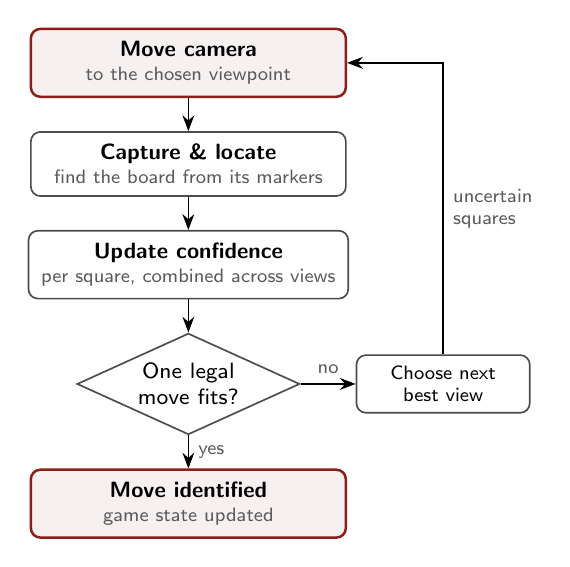
\begin{tikzpicture}[node distance=4.2mm,
  st/.style={blk,minimum width=40mm,inner sep=1.6mm},
  side/.style={blk,minimum width=22mm,inner sep=1.4mm,font=\scriptsize}]
  \node[key,minimum width=40mm,inner sep=1.6mm] (a) {\bt{Move camera}{to the chosen viewpoint}};
  \node[st,below=of a] (b) {\bt{Capture \& locate}{find the board from its markers}};
  \node[st,below=of b] (c) {\bt{Update confidence}{per square, combined across views}};
  \node[dec,below=of c] (d) {One legal\\move fits?};
  \node[key,minimum width=40mm,inner sep=1.6mm,below=of d] (e) {\bt{Move identified}{game state updated}};
  \node[side,right=7mm of d] (f) {Choose next\\best view};
  \draw[arr] (a)--(b); \draw[arr] (b)--(c); \draw[arr] (c)--(d);
  \draw[arr] (d)--node[right,sub]{yes}(e);
  \draw[arr] (d)--node[above,sub]{no}(f);
  \draw[arr] (f) |- node[sub,pos=0.25,right,align=left]{uncertain\\squares} (a);
\end{tikzpicture}
\captionof{figure}{Active board reading}\label{fig:vision}
\end{center}

\subsection{Detecting the Player's Move}
The robot does not need to be certain about all 64 squares. It already knows the previous
position, so the player can only have made one of about 20 to 40 legal moves. Each of those
moves predicts a change to just two to four squares. The robot keeps looking only until the
evidence picks out one of those moves clearly, and it chooses views that best tell the remaining
candidates apart.

As a result, most turns need only one or two views, and difficult positions get more. The robot
never has to recognise which piece is which, because the game history already tells it.
If no legal move fits, or the position is still unclear after four views, the game pauses
and the player is asked to check the board.

\subsection{Choosing a Reply}
The robot's reply is chosen by Stockfish, one of the strongest chess engines available.
The difficulty can be set before each game, from beginner level, where the engine
deliberately makes mistakes, up to full strength.

\subsection{Motion Planning}
The robot knows where the board, the camera, the arm base and the gripper are relative to
each other. It uses this to convert a square on the board into joint angles for the arm. Every
movement is checked against the arm's safe range before it is sent to the servos.
Each pick-and-place follows the same eight-step sequence (Figure~\ref{fig:pick}).

\begin{center}
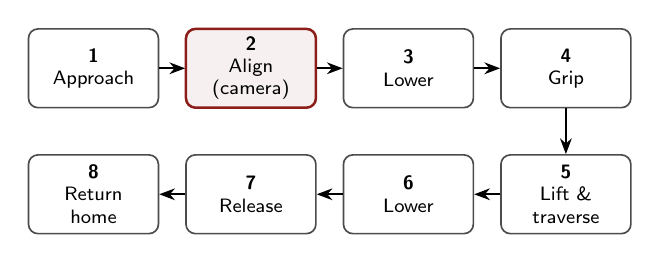
\begin{tikzpicture}[x=1mm,y=1mm,
  s/.style={blk,minimum width=16.5mm,minimum height=10mm,inner sep=0.8mm,font=\scriptsize}]
  \foreach \n/\t/\x/\y in {1/Approach/0/0, 2/Align\\(camera)/20/0, 3/Lower/40/0, 4/Grip/60/0,
                           5/Lift \&\\traverse/60/-16, 6/Lower/40/-16, 7/Release/20/-16, 8/Return\\home/0/-16}{
    \node[s] (s\n) at (\x,\y) {\textbf{\n}\\\t};
  }
  \node[key,minimum width=16.5mm,minimum height=10mm,inner sep=0.8mm,font=\scriptsize] at (20,0) {\textbf{2}\\Align\\(camera)};
  \draw[arr] (s1)--(s2); \draw[arr] (s2)--(s3); \draw[arr] (s3)--(s4);
  \draw[arr] (s4)--(s5); \draw[arr] (s5)--(s6); \draw[arr] (s6)--(s7); \draw[arr] (s7)--(s8);
\end{tikzpicture}
\captionof{figure}{Pick-and-place sequence}\label{fig:pick}
\end{center}

\subsection{Visual Grasp Alignment}
Hobby servos have some play, so the arm arrives above a square close to the target but not exactly
on it. The camera closes the gap. It measures how far the piece is from the centre of the gripper,
the arm makes a small correction, and the camera looks again. This is closed-loop visual servoing.
It normally converges to within 2\,mm in one or two corrections. If it has not converged after three,
the robot reports a fault instead of grabbing blindly.

Pieces are gripped near the top, where they are narrowest, so that the gripper fingers clear
the pieces on neighbouring squares.

\subsection{Verification and Recovery}
After placing a piece, the robot reads the board again and compares it with the
position it expects, looking closely at the squares involved in the move. If a piece is missing, misplaced or still in the gripper, it tries
again. If the second attempt fails, the arm returns home, stops and reports the problem.

\subsection{Companion Display}
The robot has no screen of its own. Instead, it serves a simple web page that opens in the
browser of any phone, tablet or computer, with nothing to install. It connects either over
Wi-Fi, or through the USB cable when the Raspberry Pi is powered from a computer.

The companion display shows:
\begin{itemize}
  \item both players' clocks: tap your side to end your turn
  \item game settings: difficulty, time control and the robot's colour
  \item the list of moves played
  \item prompts, for example \textit{``Place a queen on e8''}
  \item errors, for example \textit{``Illegal move: return the piece on e4''}
  \item faults, for example \textit{``Could not pick up the piece on g8''}
\end{itemize}

\subsection{Chess Clock}
The clock times both players. The player's clock stops when they tap it on the companion
display. The robot's clock stops once its move has been placed and verified. The game
can also be played untimed.

% ---------------------------------------------------------------------
\section{Chess Rule Support}
The chess engine makes sure every move is legal. The robot handles the physical side of
each type of move.

\begin{simpletable}{Physical handling of moves}
Ordinary move & Picks up the piece and places it on its new square\\
Capture       & Moves the captured piece to the capture tray first, then makes the move\\
Castling      & Moves the king, then the rook\\
En passant    & Removes the captured pawn, then moves the capturing pawn\\
Promotion     & Removes the pawn; the player places the new piece when prompted\\
Illegal move  & Pauses and shows which square needs correcting\\
\end{simpletable}

% ---------------------------------------------------------------------
\section{Hardware}
\begin{simpletable}{Main components}
Computer          & Raspberry Pi Zero 2 W (512\,MB RAM)\\
Camera            & Raspberry Pi Camera Module 3, \SI{12}{MP}, autofocus\\
Camera connection & CSI ribbon cable, 22-pin to 15-pin\\
Servo controller  & PCA9685, 16-channel PWM, connected over I\textsuperscript{2}C\\
Robotic arm       & 6DOF metal arm: five joints plus gripper\\
Actuators         & Six servo motors (rated \SIrange{4.8}{7.2}{V})\\
Gripper           & Two-finger claw\\
Storage           & microSD card\\
Board markers     & Printed ArUco markers around the board edge\\
\end{simpletable}

% ---------------------------------------------------------------------
\section{Specifications}
Typical values for the complete system. These will be updated with measured results as testing
is completed.

\begin{simpletable}{Physical}
Footprint           & 420 $\times$ 260\,mm (board and arm base)\\
Height              & 380\,mm (arm in home position)\\
Weight              & 2.6\,kg (without pieces)\\
Board               & 224 $\times$ 224\,mm, 28\,mm squares\\
Pieces              & Staunton, base up to 20\,mm, height up to 60\,mm\\
\end{simpletable}

\begin{simpletable}{Arm and gripper}
Joints              & 5 joints plus gripper (6 servos)\\
Maximum reach       & 400\,mm, fully extended\\
Working reach       & About 280\,mm with the gripper pointing down\\
Payload             & 150\,g at full reach\\
Gripper opening     & 0--55\,mm\\
Joint speed limit   & 60\,$^\circ$/s (set in software)\\
\end{simpletable}

\begin{simpletable}{Electrical}
Raspberry Pi supply & 5\,V USB, 2.5\,A adapter\\
Servo supply        & 6\,V regulated, rated 10\,A\\
Servo current       & About 2.5\,A while moving\\
Peak servo current  & Up to 7.5\,A\\
\end{simpletable}

\begin{simpletable}{Vision}
Board location      & Printed markers around the board edge\\
Views per board read & 1--4, typically 1--2\\
Board read time     & About 3--10\,s, depending on views\\
Grasp alignment     & Up to 3 corrections, to within 2\,mm\\
Lighting            & Even, at least 300\,lux\\
\end{simpletable}

\begin{simpletable}{Performance}
Placement accuracy  & $\pm$3\,mm, with visual correction\\
Repeatability       & $\pm$5\,mm, without visual correction\\
Pick-and-place      & 98\,\% succeed first time\\
Engine reply        & 1--5\,s, depending on difficulty\\
Ordinary move       & About 25\,s\\
Capture             & About 40\,s\\
Start-up            & About 45\,s to ready\\
\end{simpletable}

% ---------------------------------------------------------------------
\section{Power}
The Raspberry Pi and the servos are powered separately (Figure~\ref{fig:hw}).
\begin{itemize}
  \item \textbf{Raspberry Pi}: \SI{5}{V} over USB, from a phone-style charger or a computer.
  \item \textbf{Servos}: a separate regulated \SI{6}{V} supply connected to the servo
        controller's power rail. The servos draw large currents when they start moving or
        hold a load, so they must never be powered from the Raspberry Pi.
  \item \textbf{Ground}: the Raspberry Pi, servo controller and servo supply share a common ground.
\end{itemize}
The servo supply should never exceed \SI{7.2}{V}.

% ---------------------------------------------------------------------
\section{Software}
\begin{simpletable}{Software components}
Raspberry Pi OS      & Operating system\\
Python               & Main application\\
Picamera2            & Camera control\\
OpenCV               & Marker detection, square occupancy, piece location\\
Active vision        & Confidence per square, choosing the next view\\
python-chess         & Game state and chess rules\\
Stockfish            & Move selection\\
Robot control        & Arm kinematics and motion sequences\\
Web server           & Companion display\\
\end{simpletable}
The vision software uses standard image-processing techniques rather than large AI models,
which keeps it light enough to run on the Pi Zero 2 W.

% ---------------------------------------------------------------------
\section{Setup}
\begin{enumerate}
  \item Place the arm and board on a flat table, with the arm base centred along one edge of the board.
  \item Set up the pieces and put the capture tray in place.
  \item Power the Raspberry Pi, then switch on the servo supply.
  \item Open the companion display on a phone or computer.
  \item On first use, run calibration from the companion display.
  \item Choose the difficulty, time control and colour, then start the game.
\end{enumerate}
Calibration measures the offset between the camera and the gripper, and records the arm
position above each square. Because the board markers let the robot locate the board in any
view, small knocks to the board are corrected automatically. Full calibration is only needed if
the board is moved to a new position. The board should be evenly lit, without strong shadows or glare.

% ---------------------------------------------------------------------
\section{Safety}
\begin{itemize}
  \item Keep hands away from the arm while it is moving.
  \item The servo supply has a power switch within easy reach. Switch it off before reaching into the arm's workspace.
  \item Arm speed and joint range are limited in software.
  \item The arm returns to a safe home position after every move.
  \item If anything goes wrong, the arm stops and the problem is shown on the companion display.
\end{itemize}

% ---------------------------------------------------------------------
\section{Design History}

\subsection{Version 1: Magnetic Board}
\product{} began as a self-playing magnetic chessboard based on the open-source
ChessBot V1 design. A belt-driven CoreXY mechanism under the board moved an
electromagnet that dragged pieces with metal bases across the surface. An ESP32 read a grid of
64 Hall-effect sensors to detect which squares were occupied. A custom circuit board for the sensors,
motor drivers and magnet driver was designed and manufactured, and the frame was modelled for 3D printing.

\subsection{Version 2: Robotic Arm}
Dragging pieces from below has limits: pieces have to slide between other pieces, captures
are awkward, and the sensors can tell that a square is occupied but not which piece is on it.
The design was therefore changed to a robotic arm that lifts pieces from above, with a camera to guide
it. As a result, the robot no longer needs a special board or magnetic pieces.

\subsection{Hall-Sensor Board}
The original Hall-sensor board was considered as a second way of checking moves, mounted
underneath the playing surface. The camera proved reliable enough on its own, and dropping
the sensor board removed a second controller, extra wiring and an extra calibration step.

\subsection{Development Approach}
The arm version was built in stages, so that each part could be tested before the next was
added: assembling the arm, setting up the Pi and camera, detecting the board, testing the servos
one at a time, positioning the arm, grasping a piece, full pick-and-place, connecting the chess
engine, and finally verification and special moves.

% ---------------------------------------------------------------------
\section{Acknowledgements}
Version 1 is based on ChessBot V1 by Joshua Stanley Robotics (MIT License). Stockfish is
free software licensed under GPLv3.

\textbf{Use of AI.} This is a personal project, and AI tools (Anthropic's Claude) were used
throughout as a design and writing assistant. They helped plan the system architecture,
review the design for feasibility, and draft and typeset this document. The design decisions,
hardware build and testing are my own.

\end{multicols}
\end{document}
